\documentclass{article}
\usepackage[utf8]{inputenc}
\usepackage{caption}
\usepackage{amsmath}
\usepackage{amssymb}
\usepackage{mathtools}
\usepackage{multicol}
\usepackage{graphicx}
\usepackage{wrapfig}
\usepackage{float}
\usepackage[makeroom]{cancel}
\usepackage{mhchem}
\usepackage{pst-plot}

\graphicspath{ {../images/} }

\renewcommand{\familydefault}{\sfdefault}
\renewcommand{\baselinestretch}{1.5} % line spacing
\newcommand{\fline}{\par\noindent\rule{\textwidth}{0.1pt}} % horizontal line (wide)

\title{Topic 4 Acids \& Bases\\Lesson 4 - Weak and Strong Acids}
\author{Peter Zhang}

\begin{document}

\maketitle
\tableofcontents
\newpage

% lesson 4
\section{Weak Acids}
There is a chart that has the values that help you find weaker acids or bases in the data booklet. In general, if we start off with a reaction as follows:
$$\ce{HA_{weak acid} + H2O \rightleftharpoons A- + H3O+}$$
$$K_{c} = \frac{[\ce{A-}][\ce{H3O+}]}{[\ce{HA}][\ce{H2O-}]}$$
$$K_{c}[\ce{H2O}] = \frac{[\ce{A-}][\ce{H3O+}]}{[\ce{HA}]}$$
At equilibrium, the concentration of water is so low that it becomes negligible.
$$K_{a} = \frac{[\ce{A-}][\ce{H3O+}]}{[\ce{HA}]}$$
$K_{a}$ is for dissociation of a weak acid. Still an equilibrium constant. The higher the value of $K_{a}$, the greater the dissociation - \textbf{stronger acid}. \textbf{As long as $K_{a}$ exists}, it is a \textbf{weak acid}. $K_{w}$ is used when it is just water?


\section{Weak Bases}
$$\ce{B + H2O \rightleftharpoons BH+ + OH-}$$
$$K_{b} = \frac{[\ce{BH+}][\ce{OH-}]}{[\ce{B}]}$$
$K_{b}$ is the weak base dissociation constant. The higher the value the greater the \textbf{ionization}. This also means a stronger base but \textbf{THE BASE IS STILL WEAK REGARDLESS}\\
Since: $$K_{a} * K_{b} = K_{w}$$ where $K_{w} = 1*10^{-14}$ @298K and $$pKa + pKb = 14$$ we can find that the stronger acid can be found using that formula. Furthermore, using $pKa = -\log{(K_{a})}$ we can find the pH value.

\begin{figure}[H]
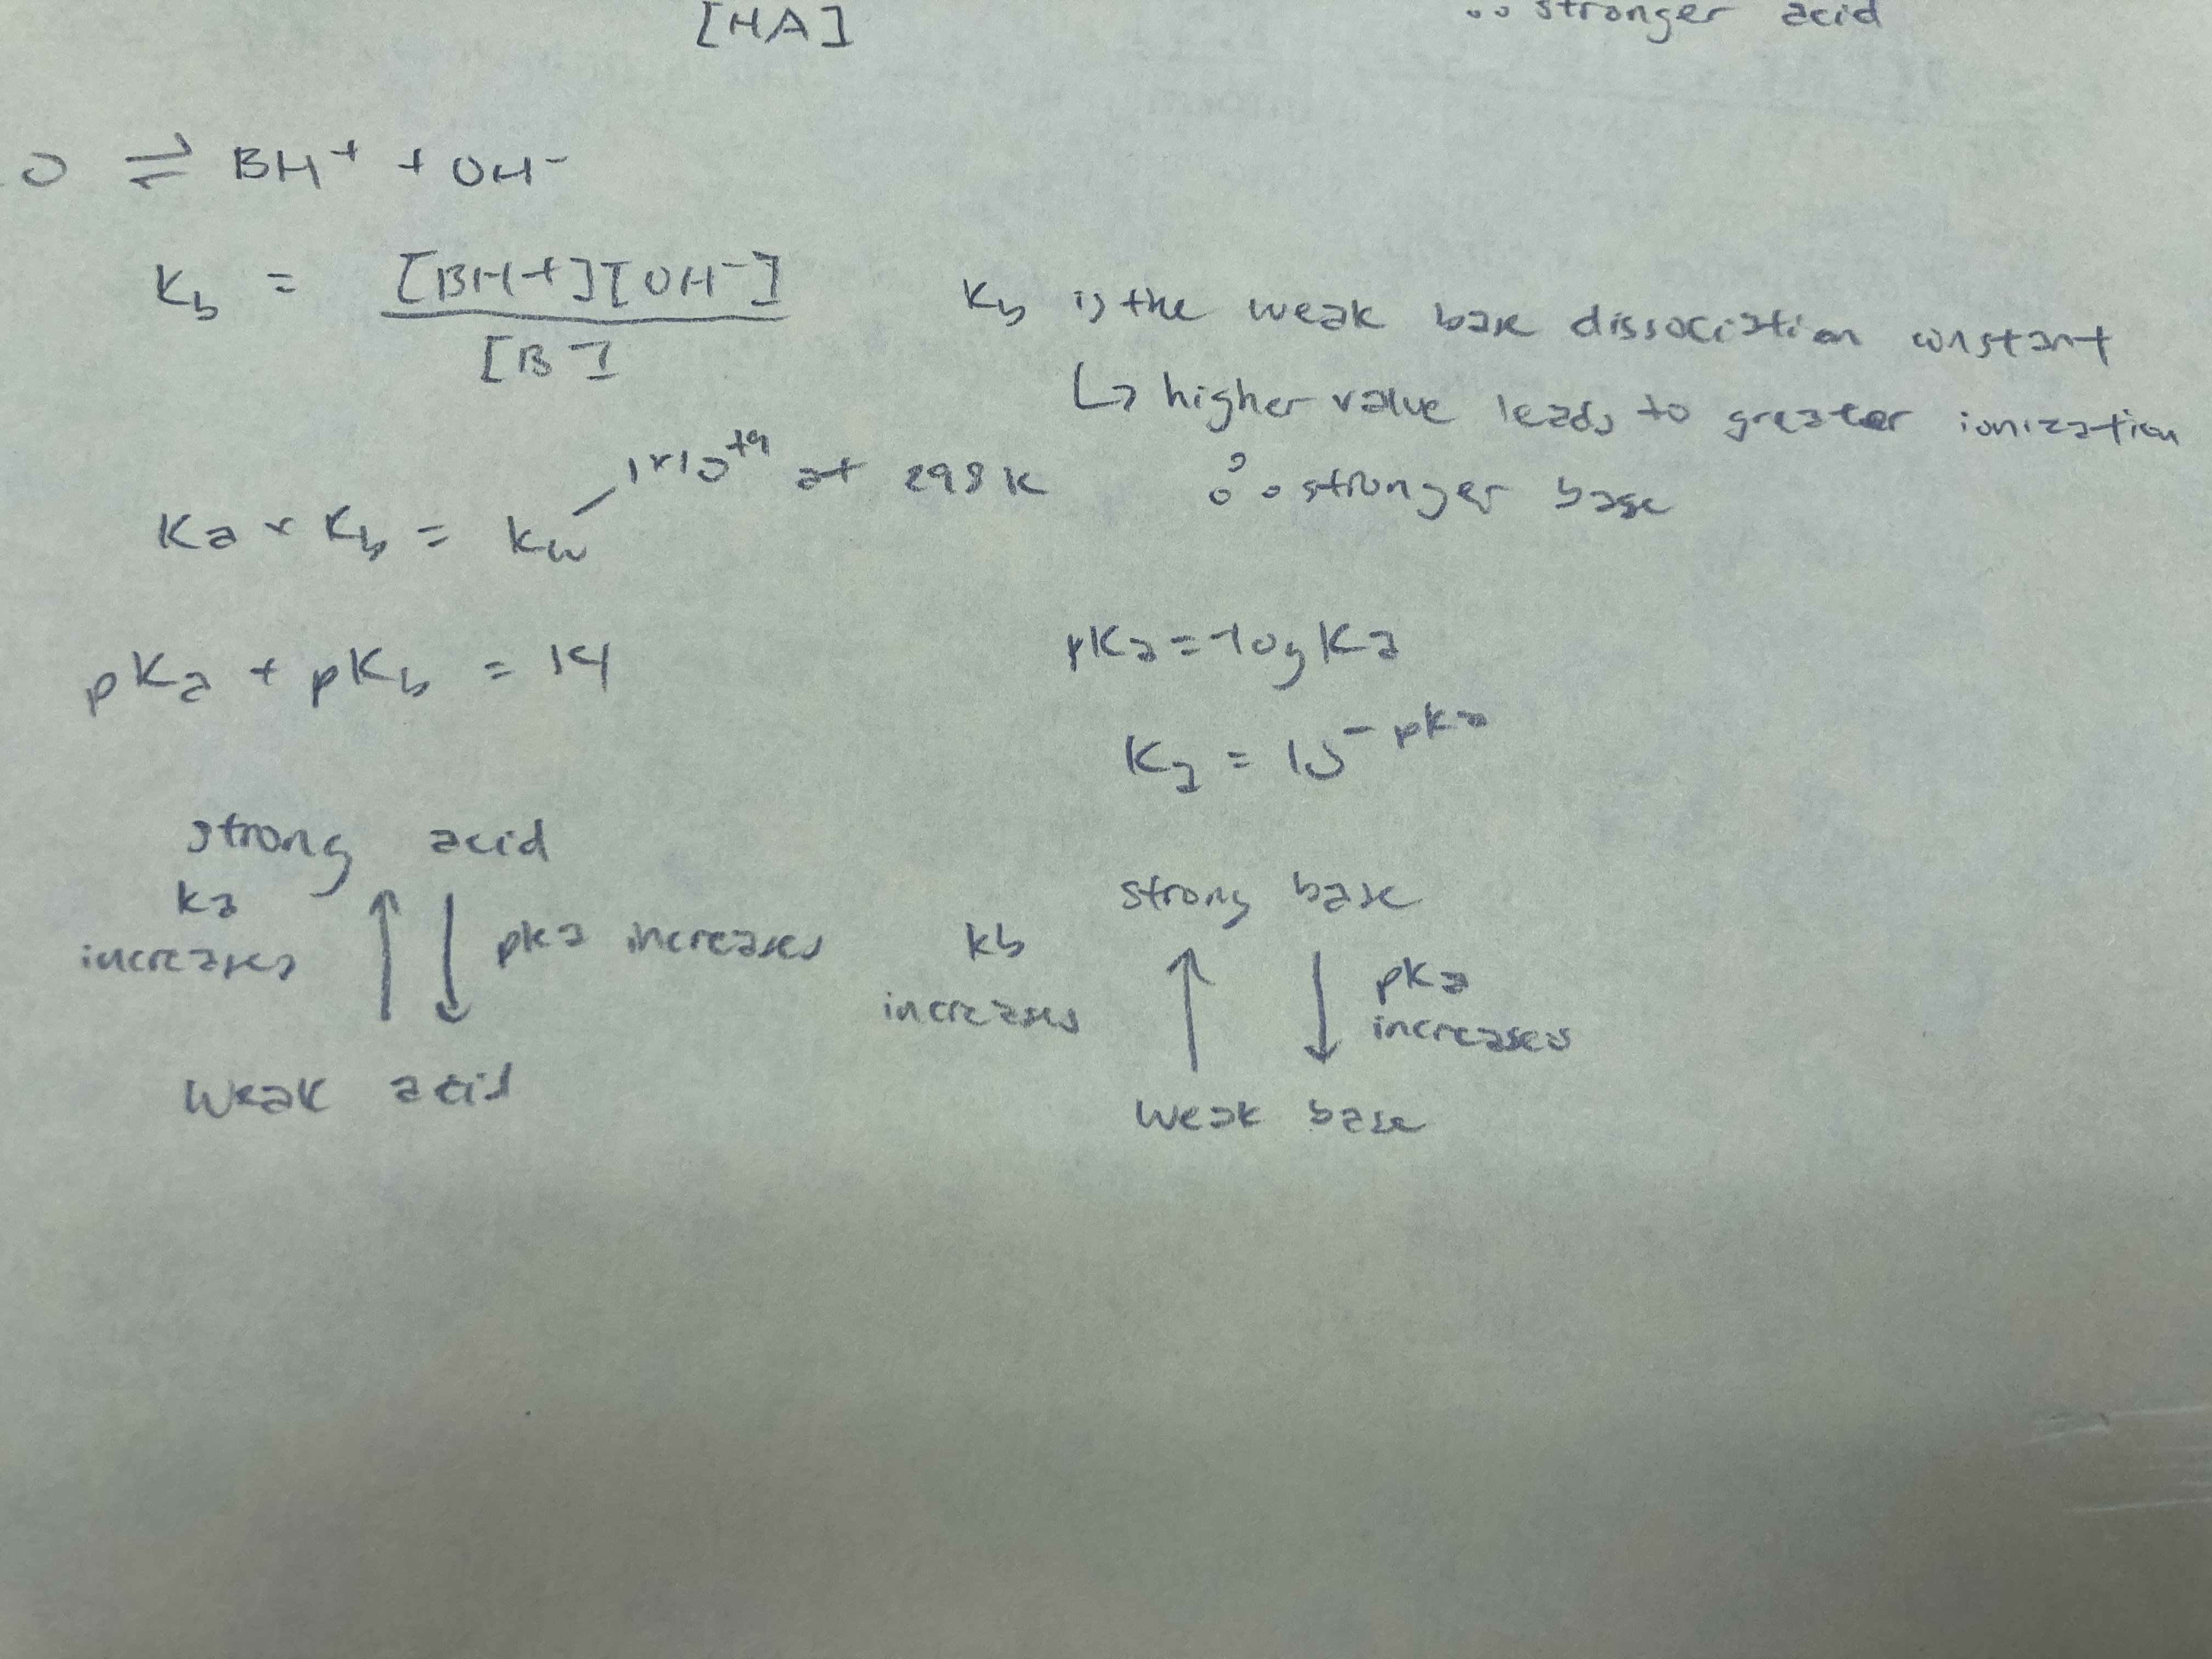
\includegraphics[width=\textwidth]{4.4fig1.jpg}
\captionof{figure}{Strong acid and Strong base diagrams}
\end{figure}


\section{Notes}
\begin{itemize}
\item using water in these reactions simplifies calculations + greater potential for reaching standards required to reach the values we have in the data booklet. If we were using a base and an acid that would somehow create some form of an exothermic reaction, the numbers would be thrown off + harder to match the actual values provided by the data booklet.
\item $K_{b}$ values can easily be converted to $K_{a}$ values. Easily switch things around just by using $$K_{a} * K_{b} = K_{w}$$ where $K_{w} = 1*10^{-14}$ @298K.
\item If you have a \textbf{STRONG} acid or base, you can just use $14 = pH + pOH$ instead of solving for these weird weak acid/base $K_{a}$ or $K_{b}$ values.
\end{itemize}


\section{Examples}
\begin{enumerate}
\item Calcualte $K_{b} + K_{a}$ for a $0.14 mol dm^{-3}$ solution of \ce{NH4} at 298K.\\It's pH is 10.43. \textbf{We must know at least one pH or pOH value}. 

$$\ce{NH3 + H2O \rightleftharpoons NH4+ + OH-}$$
We know that $14 = pH + pOH$:
\begin{align*}
pOH &= 14 - 10.43\\
&= 3.57\\
\ce{[OH-]} &= 10^{-pOH}\\
&= 10^{-3.57}\\
&= 2.69 * 10^{-4}
\end{align*}

We can then also find using weak base equilibrium formula the $K_{b}$.
\begin{align*}
K_{b} &= \frac{[\ce{NH4+}][\ce{OH-}]}{[\ce{NH3}]}\\
&= \frac{[2.69*10^{-4}]^{2}}{[\ce{NH3}]}\\
&= 5.2*10^{-2}
\end{align*}

\begin{figure}[H]
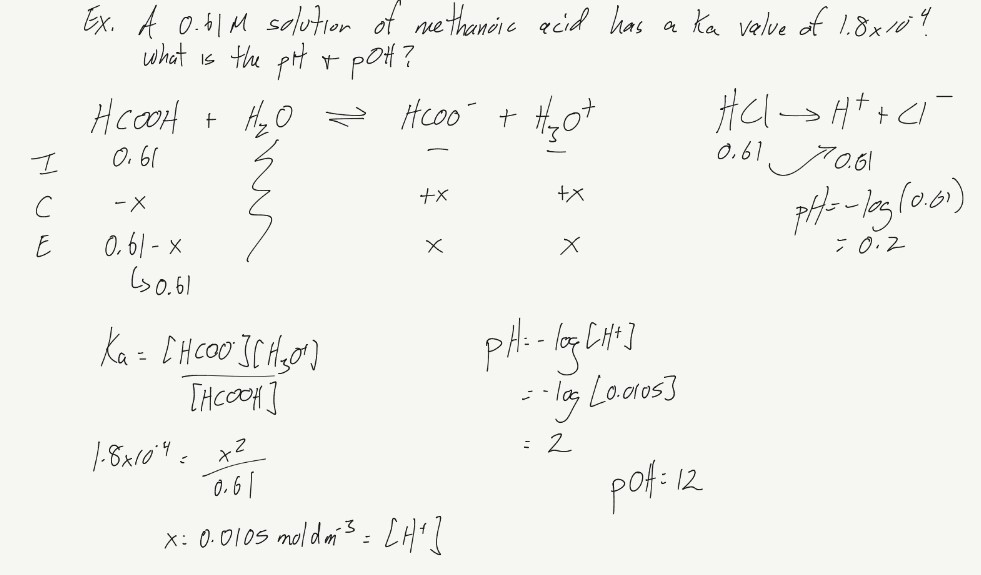
\includegraphics[width=\textwidth]{4.4ex2.jpg}
\captionof{figure}{Solution}
\end{figure}

\item A 0.61M solution of methanoic acid has a $K_{a}$ value of $1.8*10^{-4}$. What is pH + pOH?
$$\ce{HCOOH + H2O \rightleftharpoons HCOO- + H3O+}$$

\begin{figure}[H]
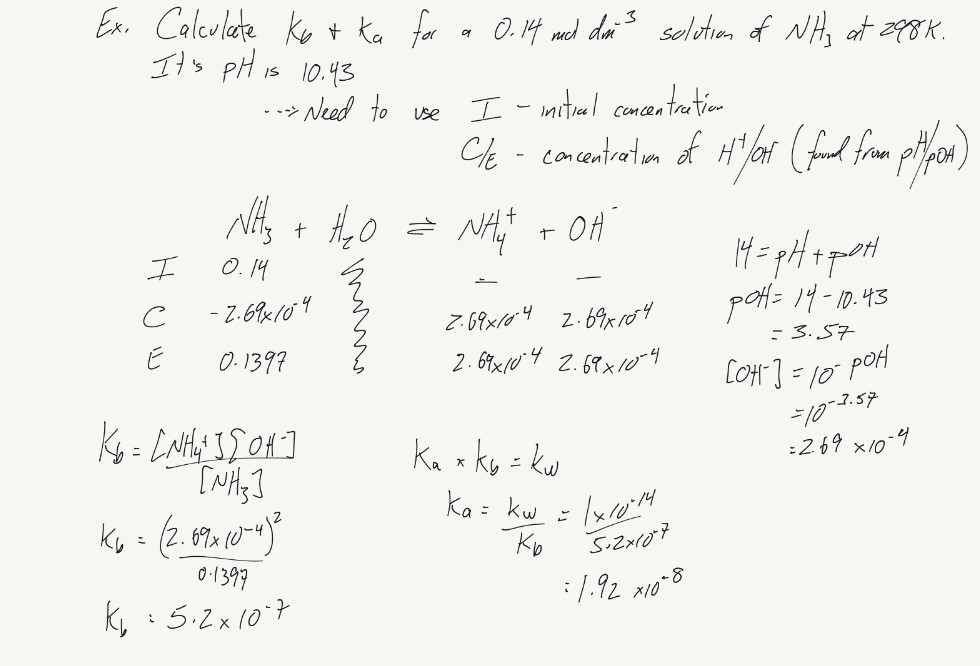
\includegraphics[width=\textwidth]{4.4ex1.jpg}
\captionof{figure}{Ice Table Solution}
\end{figure}


Solving for $K_{a}$:
\begin{align*}
K_a &= \frac{[\ce{HCOO-}][\ce{H3O+}]}{[\ce{HCOOH}]}\\
1.8*10^{-4} &= \frac{x^2}{0.61}\\
x&= 0.0105 mol dm^{-3} = [\ce{H+}]\\
\end{align*}

Solving for pH:
\begin{align*}
pH &= -\log{(\ce{H+})}\\
&= -\log{([0.0105])}\\
&= 2
\end{align*}

Therefore the pOH is 12 and the pH is 2.



\end{enumerate}















\end{document}